\section{AIS data collection}

Since the project involves simulating a maritime environment with drones, collecting real-world AIS data is crucial for creating realistic scenarios. AIS data provides information about vessel positions, speeds, and types, which can be used to populate the simulation with dynamic maritime traffic, from given time and location. This section outlines the methods for collecting AIS data, including sources, tools.

\subsection{AIS Data Sources}
Because AIS data is transmitted by vessels and received by coastal stations, there are several sources for obtaining this data:
\begin{itemize}
    \item \textbf{MarineTraffic:} A popular online platform that provides real-time and historical AIS data. It offers an paid API for accessing vessel information, which can be used to download data for specific regions and time periods.
    \item \textbf{AIS Hub:} A community-driven platform that collects AIS data from volunteers around the world. It provides free access to AIS data for research purposes, but the coverage may be limited depending on the location and the number of contributors in that area.
    \item \textbf{Local Coastal Stations:} Some coastal stations provide public access to AIS data. This can be particularly useful for collecting high-resolution data in specific areas of interest.
    \item \textbf{Homemade AIS Receiver:} Setting up a personal AIS receiver using software-defined radio (SDR) or a dedicated AIS receiver can allow for real-time data collection in the vicinity of the project location.
\end{itemize}


\begin{figure}[htbp]
    \centering
    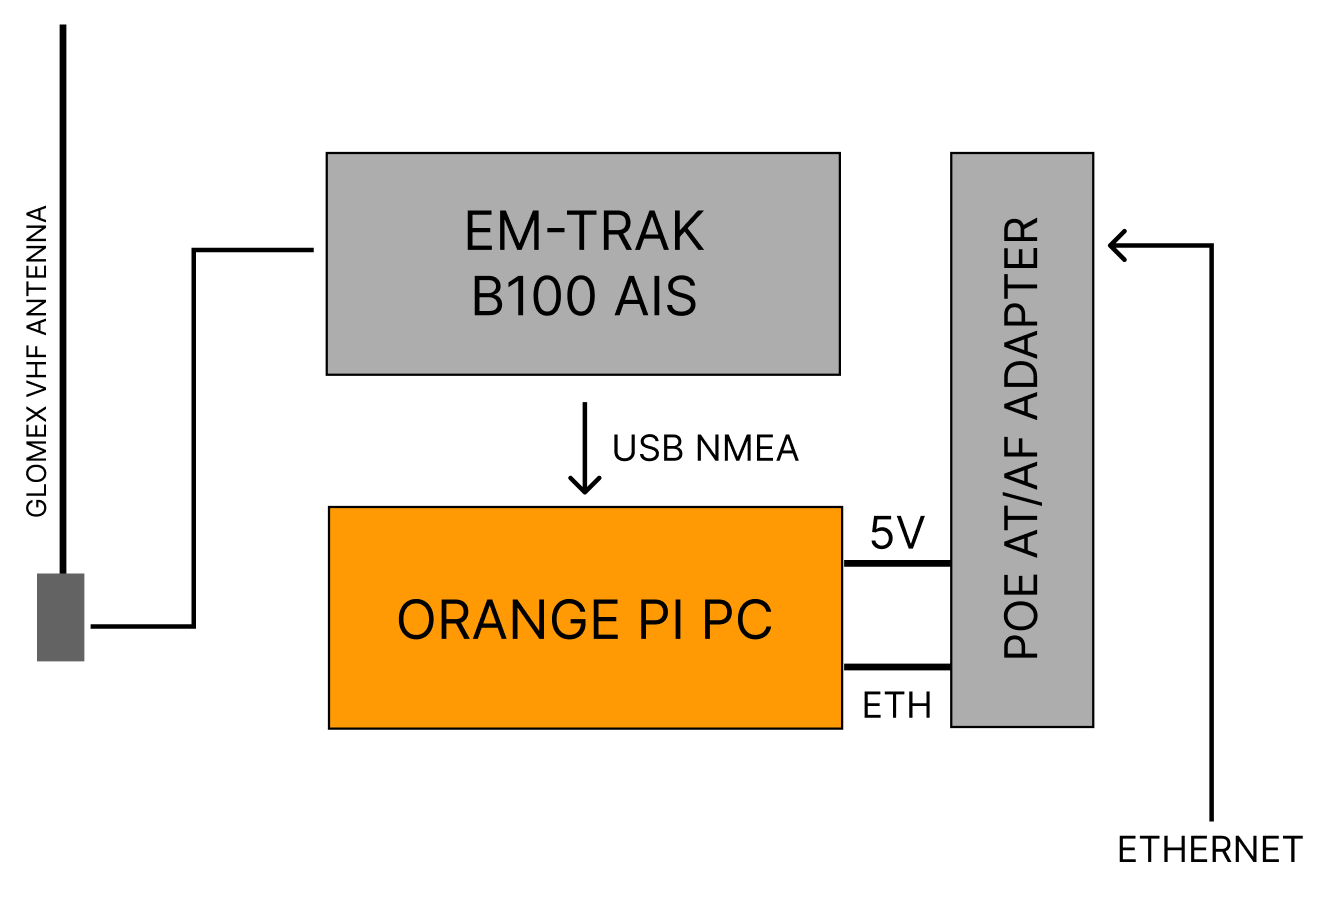
\includegraphics[width=0.6\textwidth]{images/AIS_RX_subsystems.png}
    \caption{My homemade AIS receiver system diagram.}
    \label{fig:AIS_RX_system}
\end{figure}

\vspace{0.5cm}

Since I live close to the coast, I have set up a personal AIS receiver using a
\textbf{EM-TRAK B100 AIS} receiver connected to a Orange Pi PC running custom suftware to log AIS messages, upload them to local database and visualize them on a web interface. This allows for continuous data collection and the ability to capture local maritime traffic patterns relevant to the simulation. Both AIS receiver and Orange Pi are powered by POE 802.3 at/af, which allows for easy installation and maintenance. Whole system is shown in figure \ref{fig:AIS_RX_system}. 




\vspace{0.5cm}


On a Orange Pi, I have developed a custom software that listens to the AIS receiver's output, parses the NMEA sentences, and stores the relevant data (such as MMSI, position, speed, course) in a local database. To visualize the collected AIS data, I have created a web interface that displays the positions of nearby vessels on a map in real-time. As a map I am using OpenStreetMap with Leaflet overlayer. This setup allows me to monitor maritime traffic in my area and collect data for use in the simulation environment. This system provides me a log of AIS messages in a .csv format, which can be easily imported into the simulation for creating scenarios. 

Orange Pi is running under Armbian OS, which is a lightweight Linux distribution optimized for ARM-based single-board computers. The collected AIS data is structured in a CSV format, with fields such as timestamp, MMSI, vessel name, ship type, latitude, longitude, speed in knots, and course in degrees. An example of the exported AIS data is shown in Listing \ref{lst:ais_csv_export}.

\vspace{0.5cm}

\begin{figure}[htbp]
    \centering
    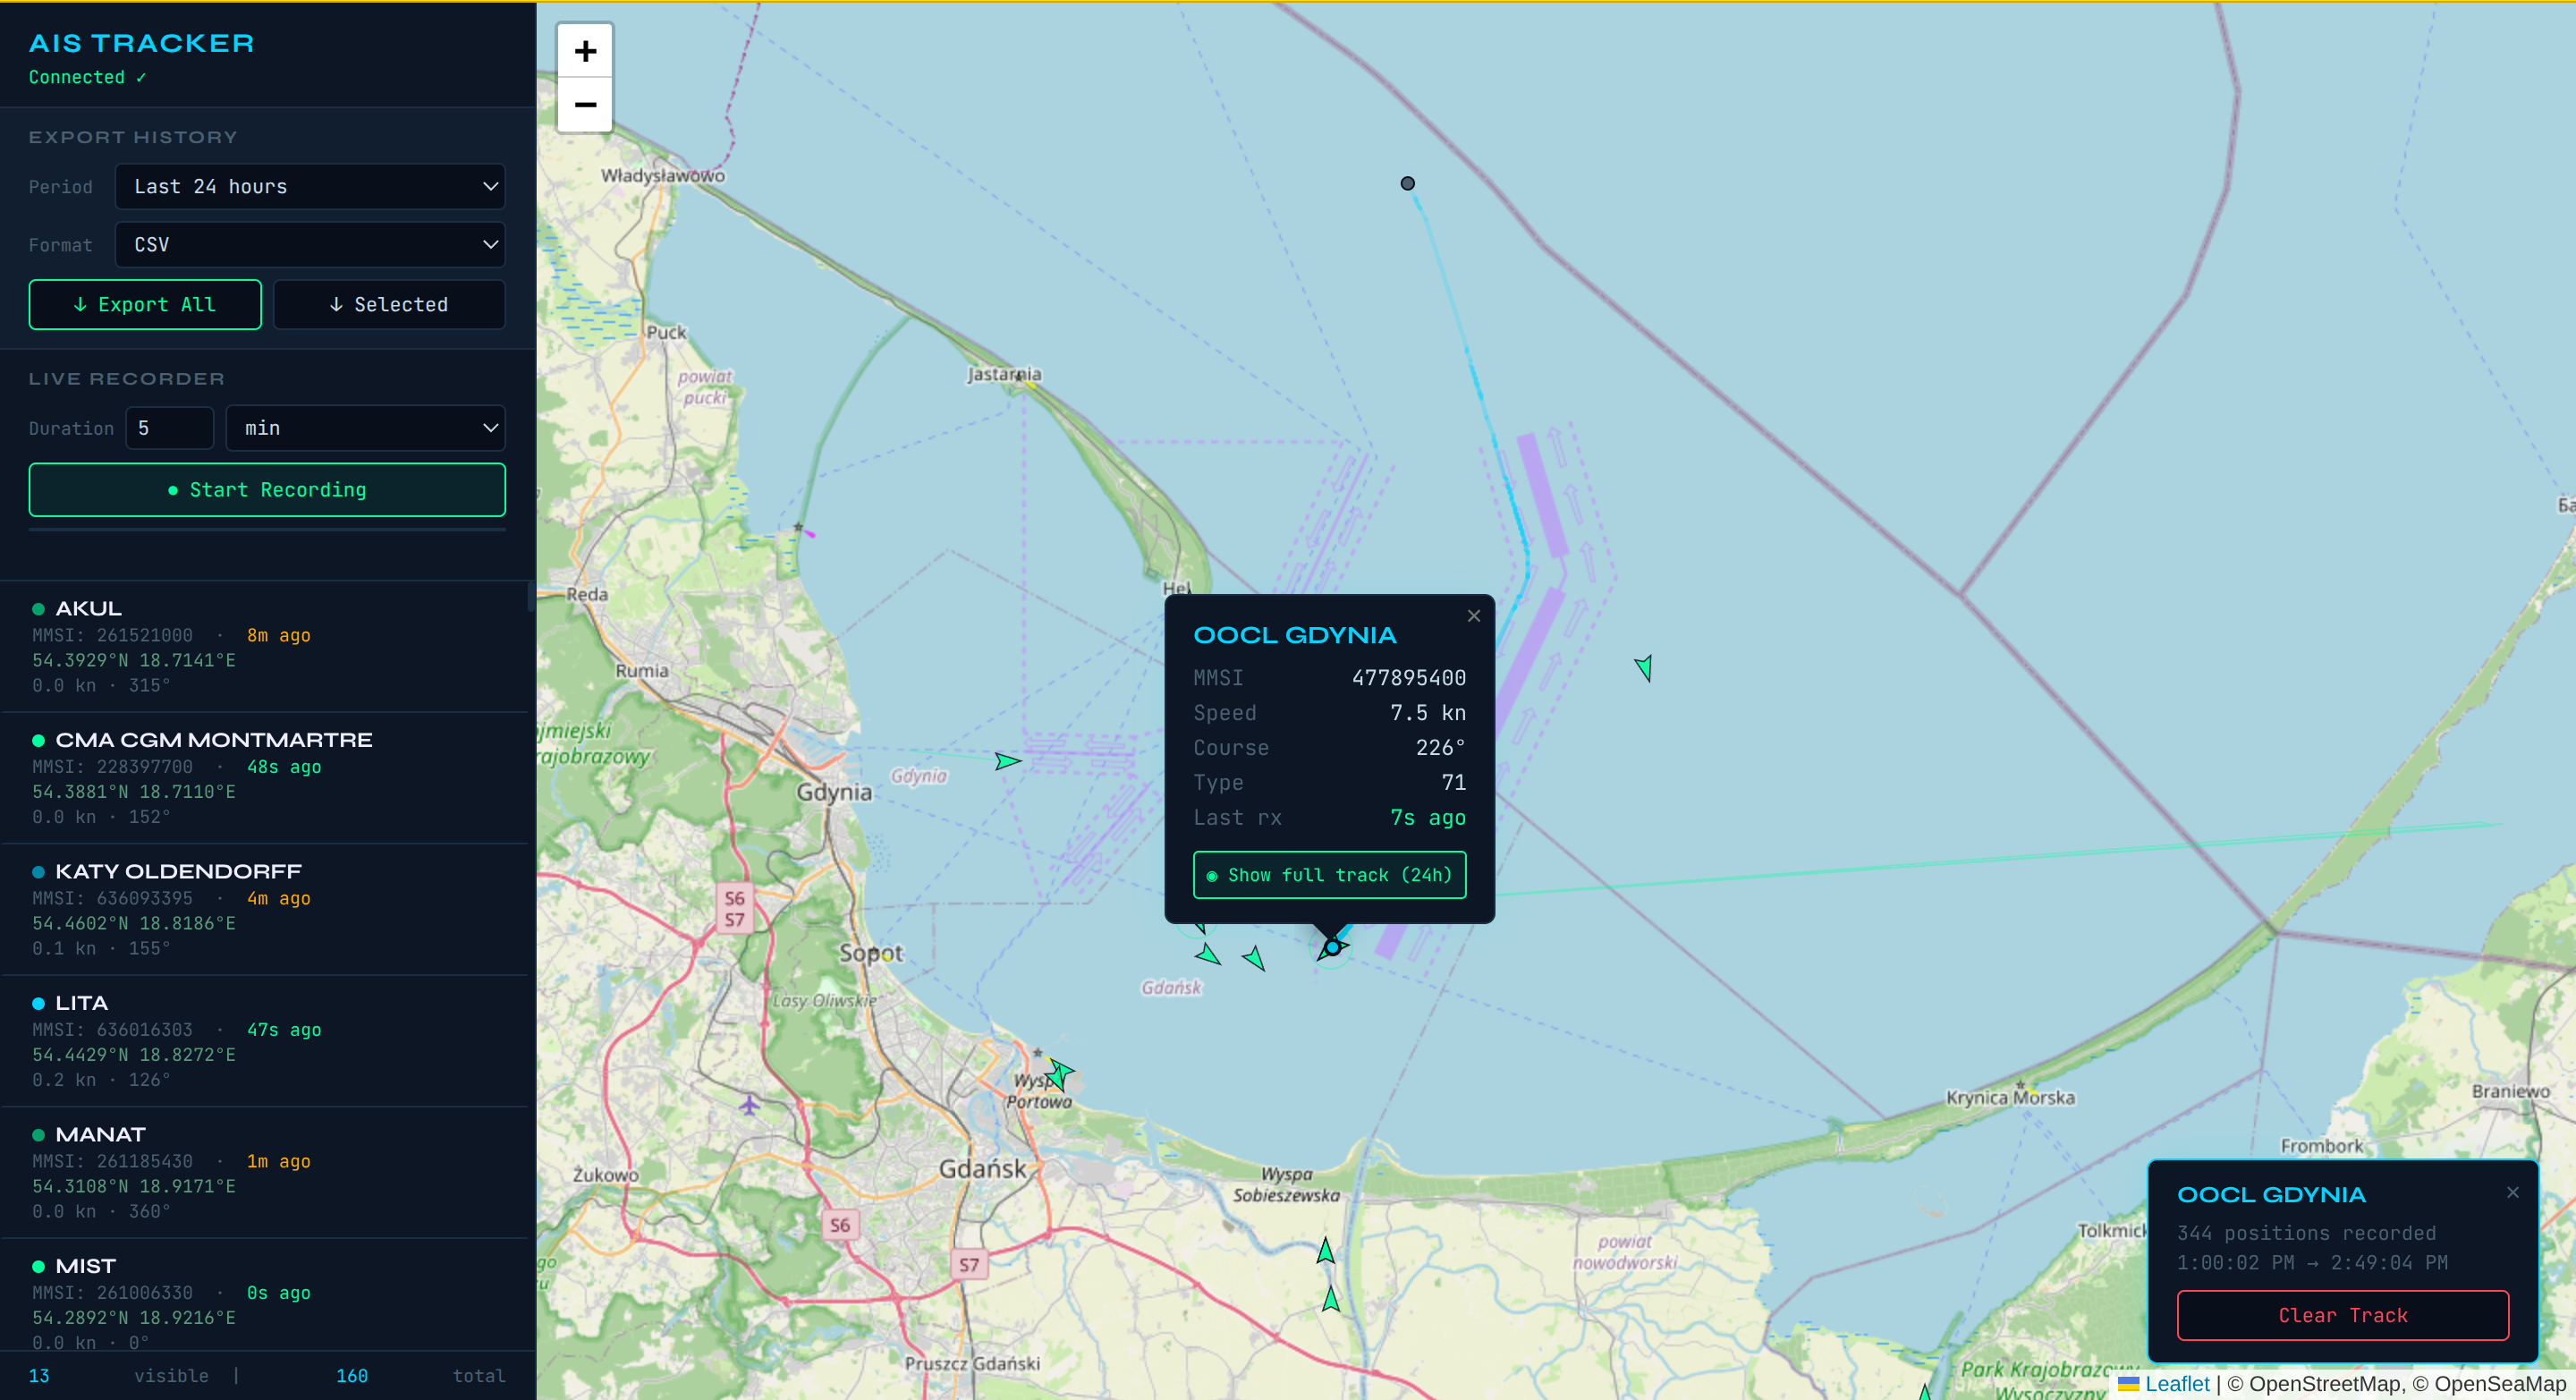
\includegraphics[width=1.0\textwidth]{images/AIS_website.png}
    \caption{My AIS data visualization web interface showing nearby vessels in real-time.}
    \label{fig:AIS_website}
\end{figure}

\vspace{0.5cm}

\subsection{Antenna and range}

To receive AIS signals I am using standard yacht VHF antenna. Model that I use is 
 \textbf {Glomex RA112}. It is a 1,5m VHF antenna with a gain of 3dB. Antenna is mounted on the roof of my house, which is approximately 10m above sea level. Between sea and my home there is a forrest, where threes might be blocking signals. With this setup, I am able to receive AIS signals from vessels within a range of approximately 20 nautical miles (37 km), depending on atmospheric conditions and the height of the transmitting vessel's antenna. This range allows me to capture a significant amount of maritime traffic in Gdańsk Bay, which is a busy shipping area. The collected data includes a variety of vessel types, speeds, and courses, providing a rich dataset for simulation.

\vspace{0.5cm}

 Listing \ref{lst:ais_csv_export}, shows the exported AIS data is structured in a CSV format. Each entry represents a received AIS message, identified by its MMSI.

\begin{lstlisting}[style=csvStyle, caption={Subsection of exported AIS telemetry for Oceania.}, label={lst:ais_csv_export}]
timestamp,mmsi,name,ship_type,lat,lon,speed_kn,course_deg
2026-04-26T06:59:51.06Z,261000150,OCEANIA,0,54.4128,19.0690,9.5,84.3
2026-04-26T07:00:12.55Z,261000150,OCEANIA,0,54.4129,19.0706,8.5,86.3
2026-04-26T07:00:32.17Z,261000150,OCEANIA,0,54.4130,19.0720,9.6,84.4
2026-04-26T07:00:42.79Z,261000150,OCEANIA,0,54.4130,19.0728,9.2,67.4
2026-04-26T07:01:01.91Z,261000150,OCEANIA,0,54.4131,19.0742,9.4,90.4
\end{lstlisting}

